\chapter{Sensor Linearity
\label{chap:10}}

To map the crushed gap sensor measurements to estimated forces, 
a regression to the forces as measured by the 
Linear Cutting Machine's strain gauges was used.
This method has a few limitations, the most significant
being the distance between the tested sensor and the strain gauges.
Because of the distance, the higher frequency force components will
be out of phase when compared. 
In addition to the distance, the viscous nature of the polyimide dielectric distorts the 
frequency response when the two measurements are compared.
The electronics for the sensor also contribute high frequency noise to the measurement.
For these reasons, the higher frequency components of the force are not directly correlated 
between the two systems. 
A plot of the transfer function between the measurements is shown in \hlgr{fig}.

When attempting to estimate the rock cutting forces to determine material type and tool wear, 
the problem can be relaxed to estimating average cutting force, as the differences in 
cutting force between the conditions are great.
The cutting force bandwitdth was limited to 10 Hz for the study, as this is believed to still
provide an adequeate response time while providing good averaging.
Plots of the sensor channel values and the measured force with and withoug filtering are shown in \hlgr{fig2}.

To improve the sensor design further, the results of this study can be used 
to make reccomendations for future designs. 
The capacitive steel donut with viscous polyimide filling is a useful base design
for many robotic applications. Robustness, linearity, and sensitivity are important 
paramters for any sensor design. Ways to improve each of these categories is listed in \ref{tab:improve}.
MATLAB models for the sensor designs are also included in \hlgr{appendix}. 
These models can be used to explore how design parameter changes will impact the sensor capacitance output.

\begin{table}[]
\centering
\caption{Changes to design parameters that would improve certain categories}
\label{tab:improve}
\begin{tabular}{|l|l|l|l|}
\hline
Parameter     & Robustness   & Linearity    & Sensitivity               \\ \hline
Dielectric    & Stiff, Tough & Stiff, Thick & High Permittivity, Thin   \\ \hline
Case Material & Thick, Tough & Stiff, Thick & Thin walls                \\ \hline
Sensing Area  & Large        & Large        & Small                     \\ \hline
\end{tabular}
\end{table}


The sensor is shown in \ref{fig:airgap}.
Laser weld procedure and simulation for air gap and are attached in \hlgr{appendix 2, appendix 3}.

\begin{figure}[ht]
\centering
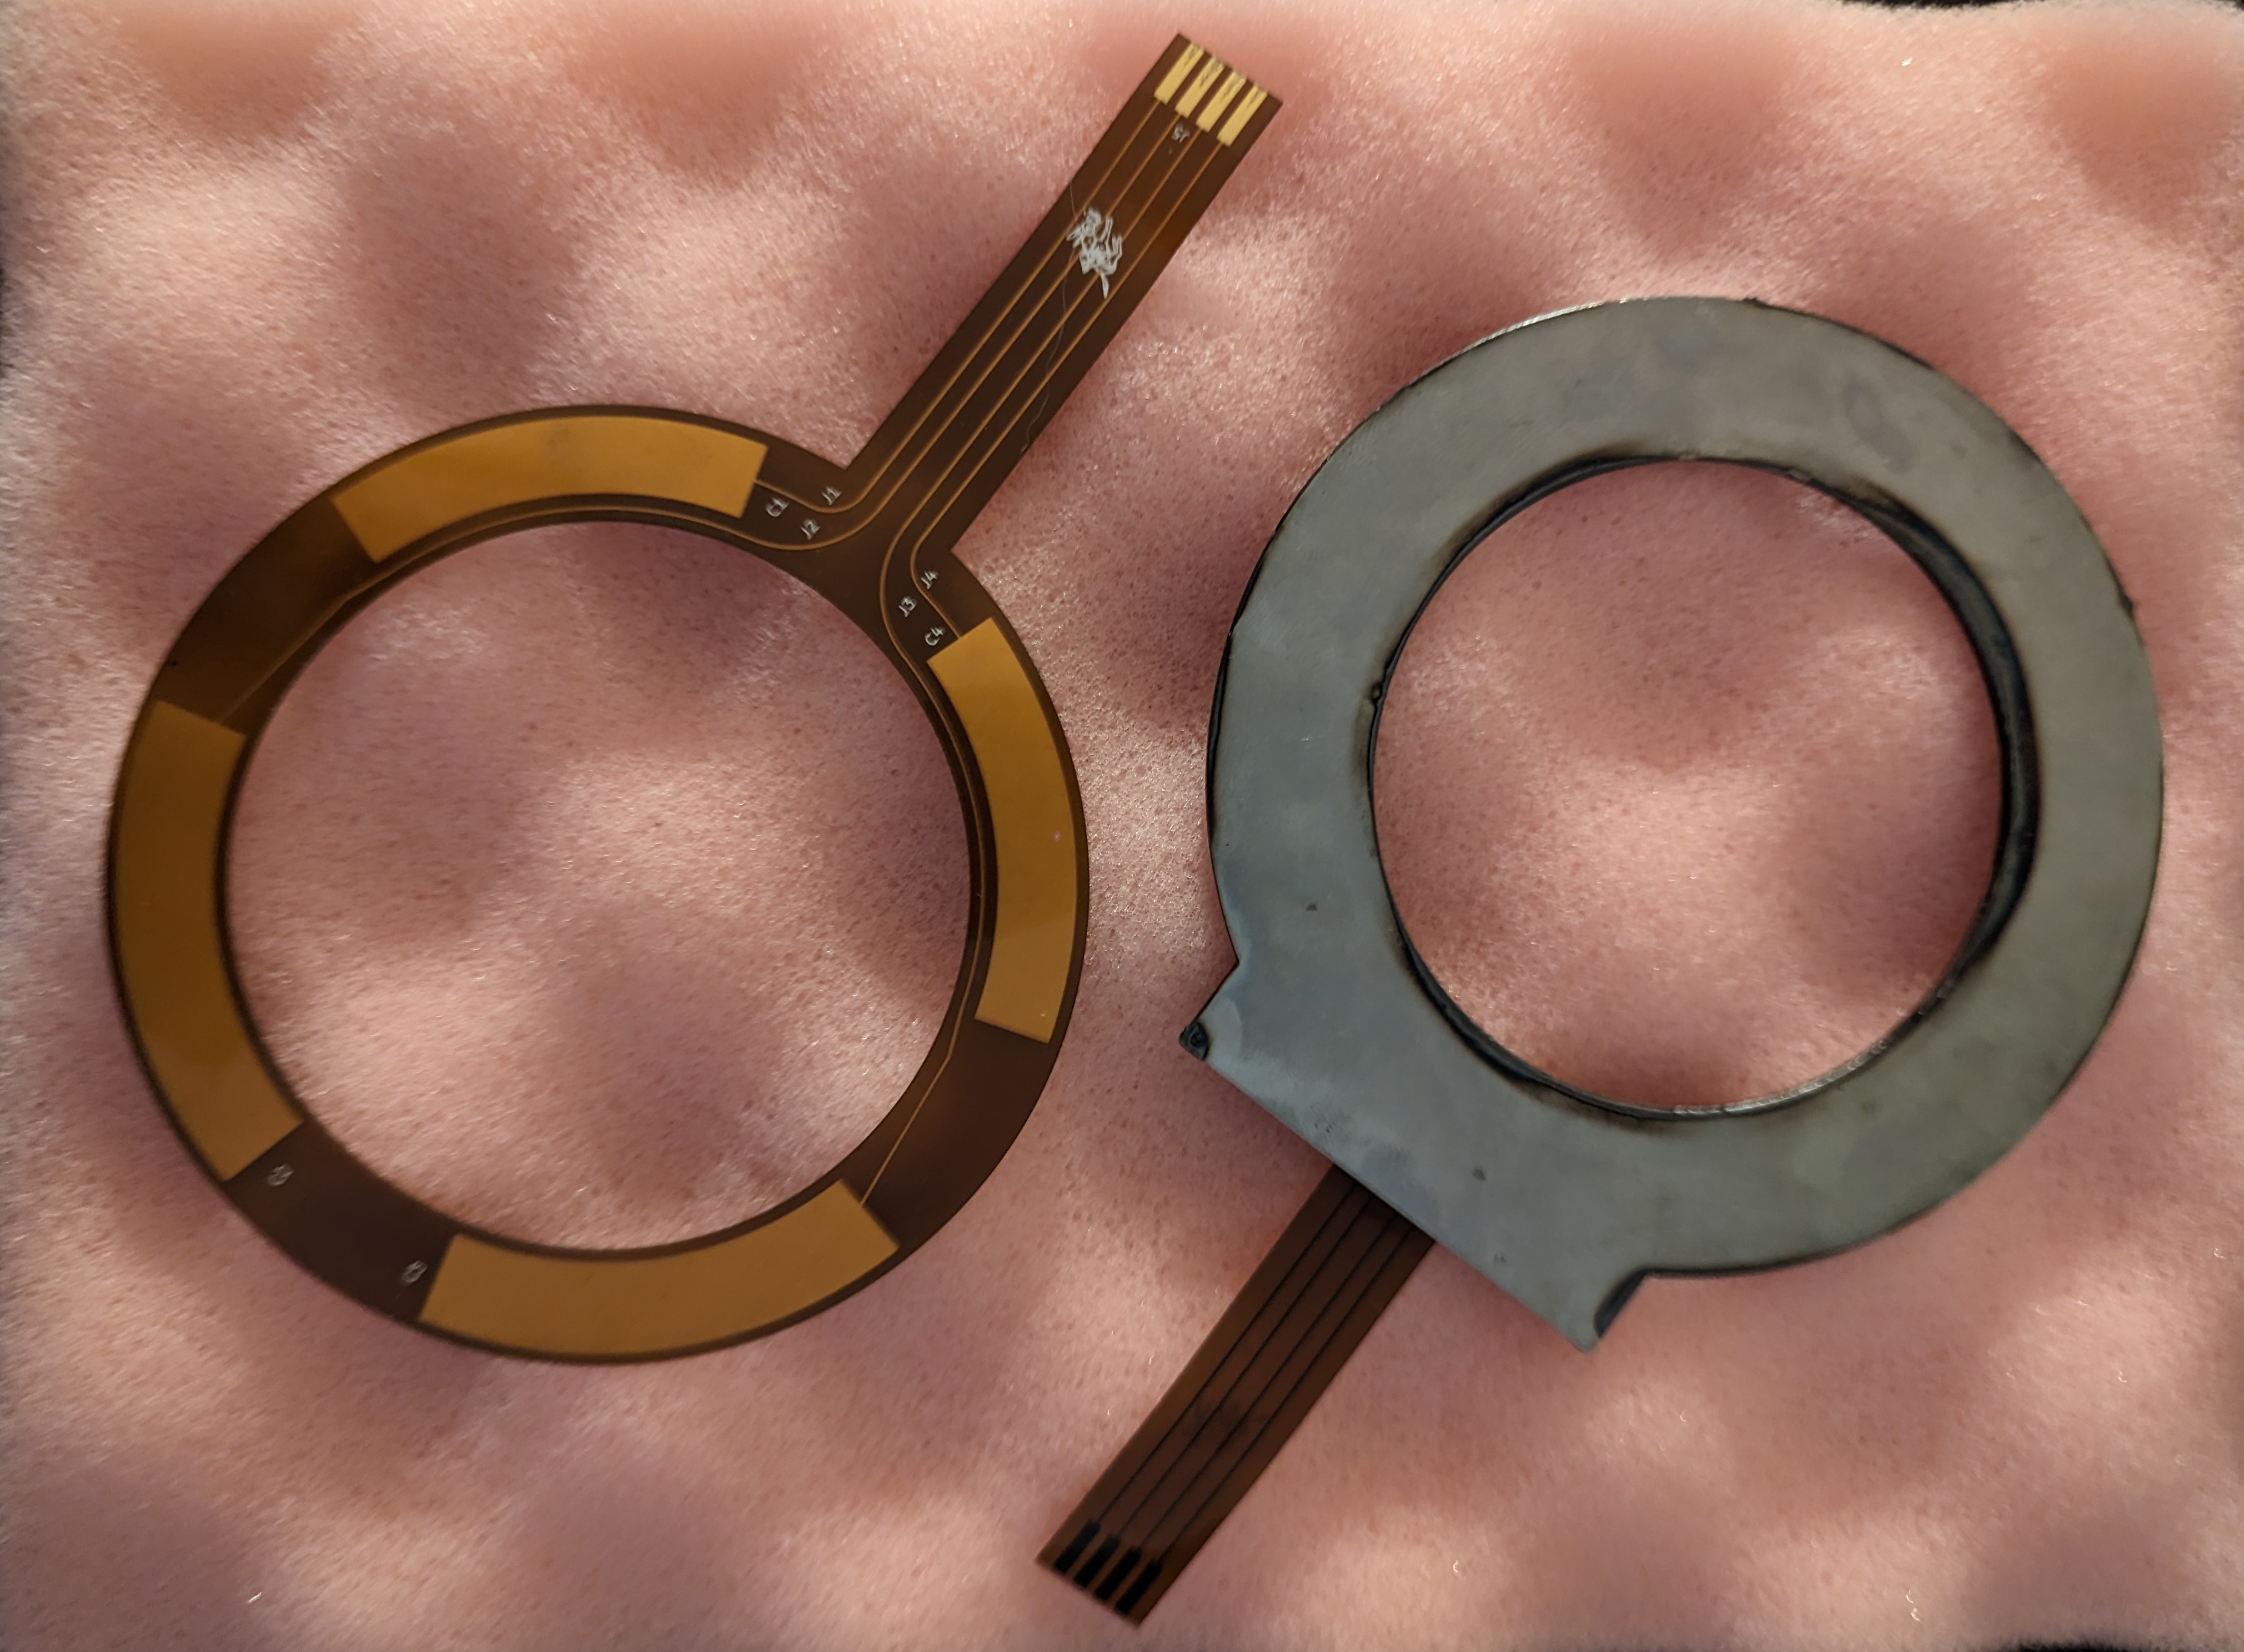
\includegraphics[width=0.7\textwidth]{airgap_and_case.jpg}
\caption{
The air gap sensor membrane, left, and an assembled prototype, right.
The sensor case provides additional protection from the environment.
The deice is assembled via later wleding.
}
\label{fig:airgap}
\end{figure}

